\documentclass[11pt]{beamer}
\usepackage[utf8]{inputenc}
\usepackage[spanish]{babel}
\usepackage{amsmath}
\usepackage{amsfonts}
\usepackage{amssymb}
\usepackage{graphicx}
\usepackage{lipsum}
\usepackage{ragged2e}
\usepackage{hyperref}
\usepackage{float}
\usepackage{url}
\usetheme{Madrid}
\newcommand{\celda}[1]{
	\begin{minipage}{2.5cm}
		\vspace{5mm}
		#1
		\vspace{5mm}
	\end{minipage}
}

\author[Erick  Ríos]{Erick Jesús Ríos González\inst{1} }
\title[TDA Liga MX]{Análisis Topologico de Datos en la Liga MX}
\date{28 de noviembre de 2024} 
\subtitle{Seminario de Topología}
\logo{
\includegraphics[scale=0.0375]{/home/soundskydriver/Documents/topological_data_analysis_mx_league/reports/presentation/images/Logo-UNAM-Azul-Landscape.png}}
\institute[UNMSM]{
	\inst{1}
		Universidad Nacional Autónoma de México. Facultad de Ciencias.
	
}

\AtBeginSection[]
{
	\begin{frame}<beamer>{Contenido}
		\tableofcontents[currentsection,currentsubsection]
	\end{frame}
}


\begin{document}
	
	\begin{frame}
		\maketitle
	\end{frame}

	\begin{frame}{Contenido}
		\tableofcontents
	\end{frame}

	\section{Resumen}
		\begin{frame}{Resumen}
			\justifying
			Realizamos un Análisis de Componentes Principales (PCA) para reducir la dimensionalidad de las estadísticas y calculamos homología persistente para estudiar las características topológicas de los datos. Además, aplicamos el algoritmo Mapper para visualizar la estructura del conjunto de datos. El análisis se centra en las estadísticas de la temporada 2023–2024 de la Liga MX, excluyendo los partidos de playoffs.

El objetivo es comprender mejor los tipos de jugadores y la distribución de su rendimiento en la liga, ofreciendo una nueva perspectiva en el análisis deportivo mediante el uso de técnicas topológicas.
		\end{frame}
	
	\section{Introducción}
    \begin{frame}
        \frametitle{Introducción}
        El análisis topológico de datos es una metodología poderosa para explorar la estructura y relaciones ocultas en conjuntos de datos complejos. En este proyecto, se utiliza para analizar el rendimiento de jugadores de fútbol en la Liga MX, utilizando datos estadísticos y técnicas de reducción de dimensionalidad. El enfoque permite descubrir patrones, similitudes y la forma topológica que subyace en los datos, lo cual es útil para la toma de decisiones y el análisis de comportamientos a través de múltiples variables.
        \end{frame}
		
	
	\section{Conocimientos Previos}
    \begin{frame}
        \subsection{Enfoque Estadístico | Componente Principal}
        \frametitle{Enfoque Estadístico: Componente Principal}
        La reducción de dimensionalidad mediante el análisis de componentes principales (PCA) permite identificar las direcciones principales de la variabilidad en los datos. Esta técnica ayuda a comprender qué variables son más importantes para describir el comportamiento de los jugadores, y a reducir la complejidad de los datos sin perder información relevante.
        \end{frame}
	
		\begin{frame}
            \frametitle{Enfoque Estadístico: Análisis de Componentes Principales (PCA)}
            El análisis de componentes principales (PCA) transforma los datos originales en un conjunto de nuevas variables ortogonales, conocidas como componentes principales, que explican la mayor parte de la varianza de los datos. Este enfoque ayuda a visualizar los datos en un espacio de menor dimensión y a identificar patrones ocultos en grandes conjuntos de datos.
            \end{frame}
        \subsection{Métodos Topológicos | Algoritmo de Mapper}
        \begin{frame}
            \frametitle{Métodos Topológicos: Algoritmo Mapper}
            El algoritmo Mapper es una herramienta poderosa en el análisis topológico de datos. Se utiliza para construir un grafo que captura la estructura de los datos, basándose en la proyección de los datos en un espacio de menor dimensión y el uso de técnicas de agrupamiento para identificar clusters de puntos de datos similares. Este grafo puede revelar la forma y las relaciones topológicas de los datos.
        \end{frame}
        \begin{frame}
            \frametitle{Métodos Topológicos: Notiones Topológicas}
            Las principales nociones topológicas aplicadas en el análisis incluyen:
            \begin{itemize}
                \item **Espacios métricos**: Representan los datos en un espacio con una métrica que define distancias entre puntos.
                \item **Clustering**: Agrupamiento de puntos en el grafo basándose en su similitud o proximidad en el espacio.
                \item **Homología persistente**: Análisis de las características topológicas de los datos en diferentes escalas.
            \end{itemize}
            Estas nociones nos ayudan a construir el grafo topológico y a interpretar su significado.
            \end{frame}
        % Slide: Topological Methods - Applying the Algorithm
    \begin{frame}
    \frametitle{Métodos Topológicos: Aplicando el Algoritmo}
    El algoritmo Mapper es aplicado a los datos reducidos a través de PCA, utilizando un algoritmo de clustering como DBSCAN. Este enfoque construye un grafo donde cada nodo representa un cluster de jugadores con características similares, y las aristas muestran las relaciones topológicas entre estos clusters.
    \end{frame}
    
    % Slide: Topological Methods - Persistent Homology
    \begin{frame}
    \frametitle{Métodos Topológicos: Homología Persistente}
    La homología persistente es una técnica que analiza la topología de los datos en varias escalas. Identifica características topológicas (como componentes conexos, ciclos y agujeros) y cómo persisten a medida que se cambia la escala del análisis. Se utiliza para entender la robustez de las estructuras detectadas en los datos.
    
    \end{frame}
	
	\section{Resultados}
		\begin{frame}{Resultados}
			\justifying
			La implementación del código para este proyecto se puede revisar en:
            \centering
            \href{https://github.com/erick-rios/topological_data_analysis_mx_league}{Topological Data Analysis League MX}
		\end{frame}
		
		\begin{frame}{Resultados}
			\justifying
			Para la primera componente principal, las variables más importantes son:
			\begin{figure}[H]
				\centering
				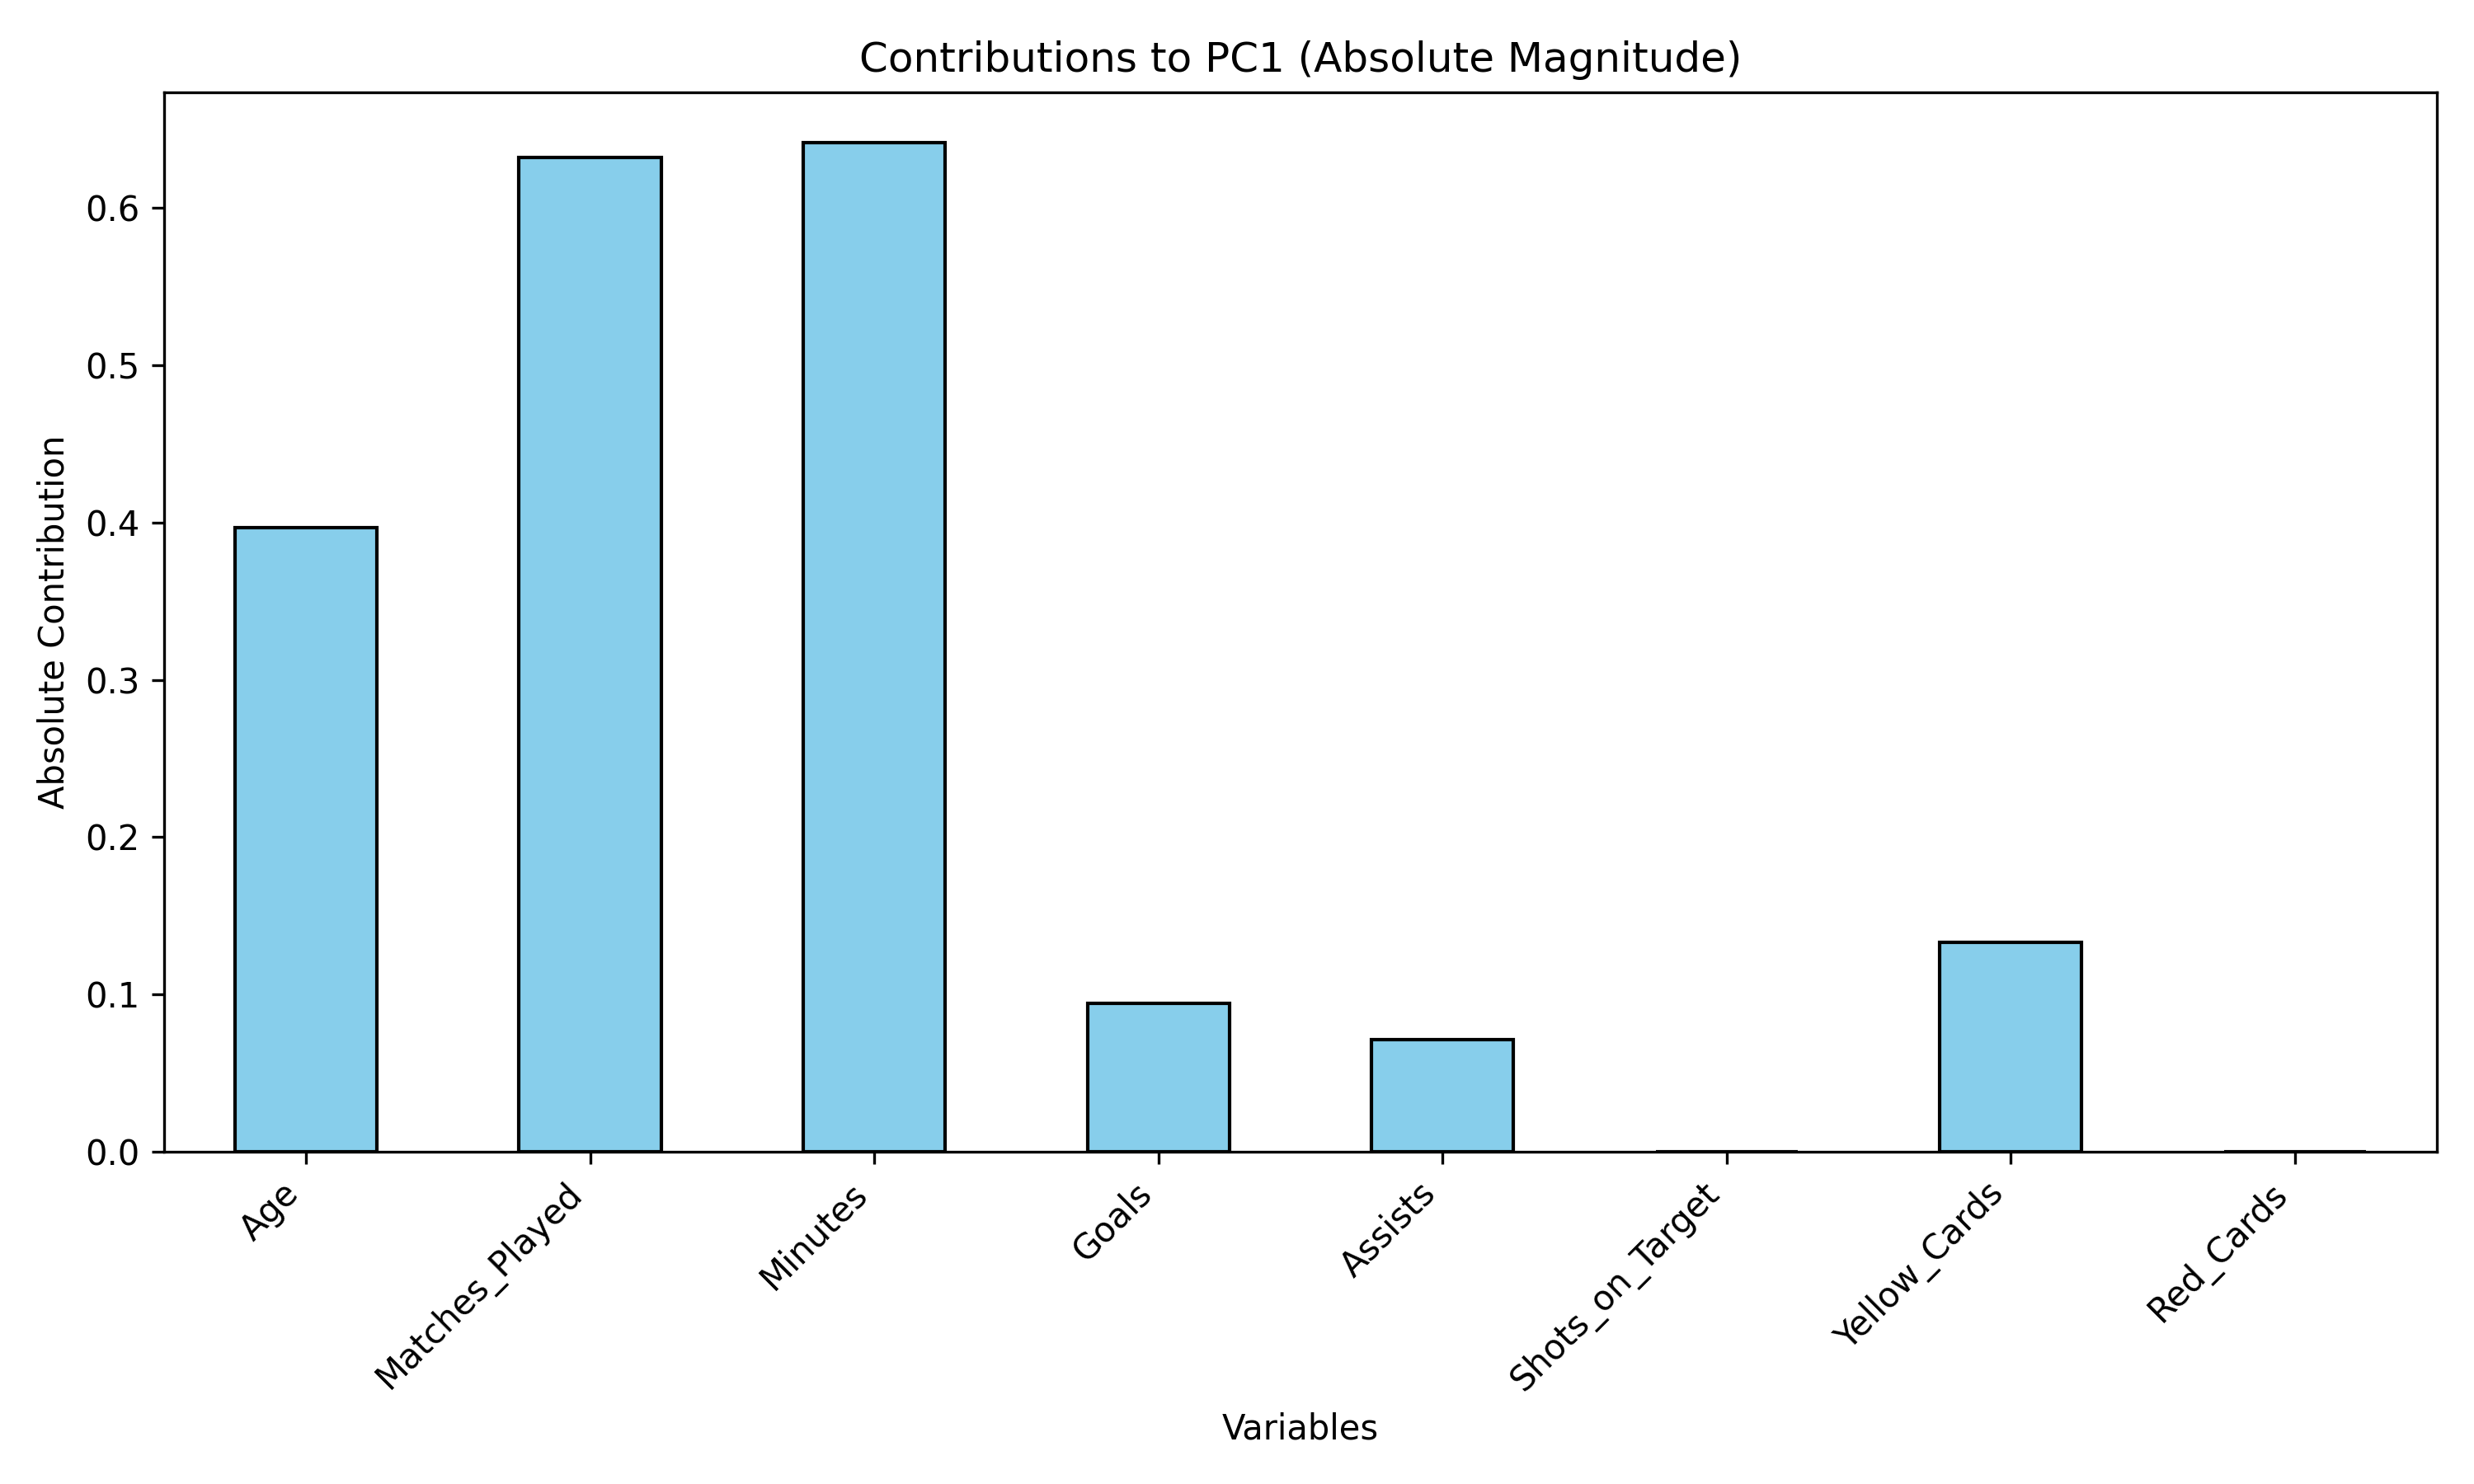
\includegraphics[scale=0.4]{/home/soundskydriver/Documents/topological_data_analysis_mx_league/reports/figures/pca_analysis/contributions_PC1_absolute.png}
				\caption{Contribuciones de las variables al primer componente principal}
                \label{fig: Figura1}
			\end{figure}
		\end{frame}
        \begin{frame}{Resultados}
			\justifying
            Mientras que para la segunda componente principal, las variables más importantes son:
            \begin{figure}[H]
				\centering
				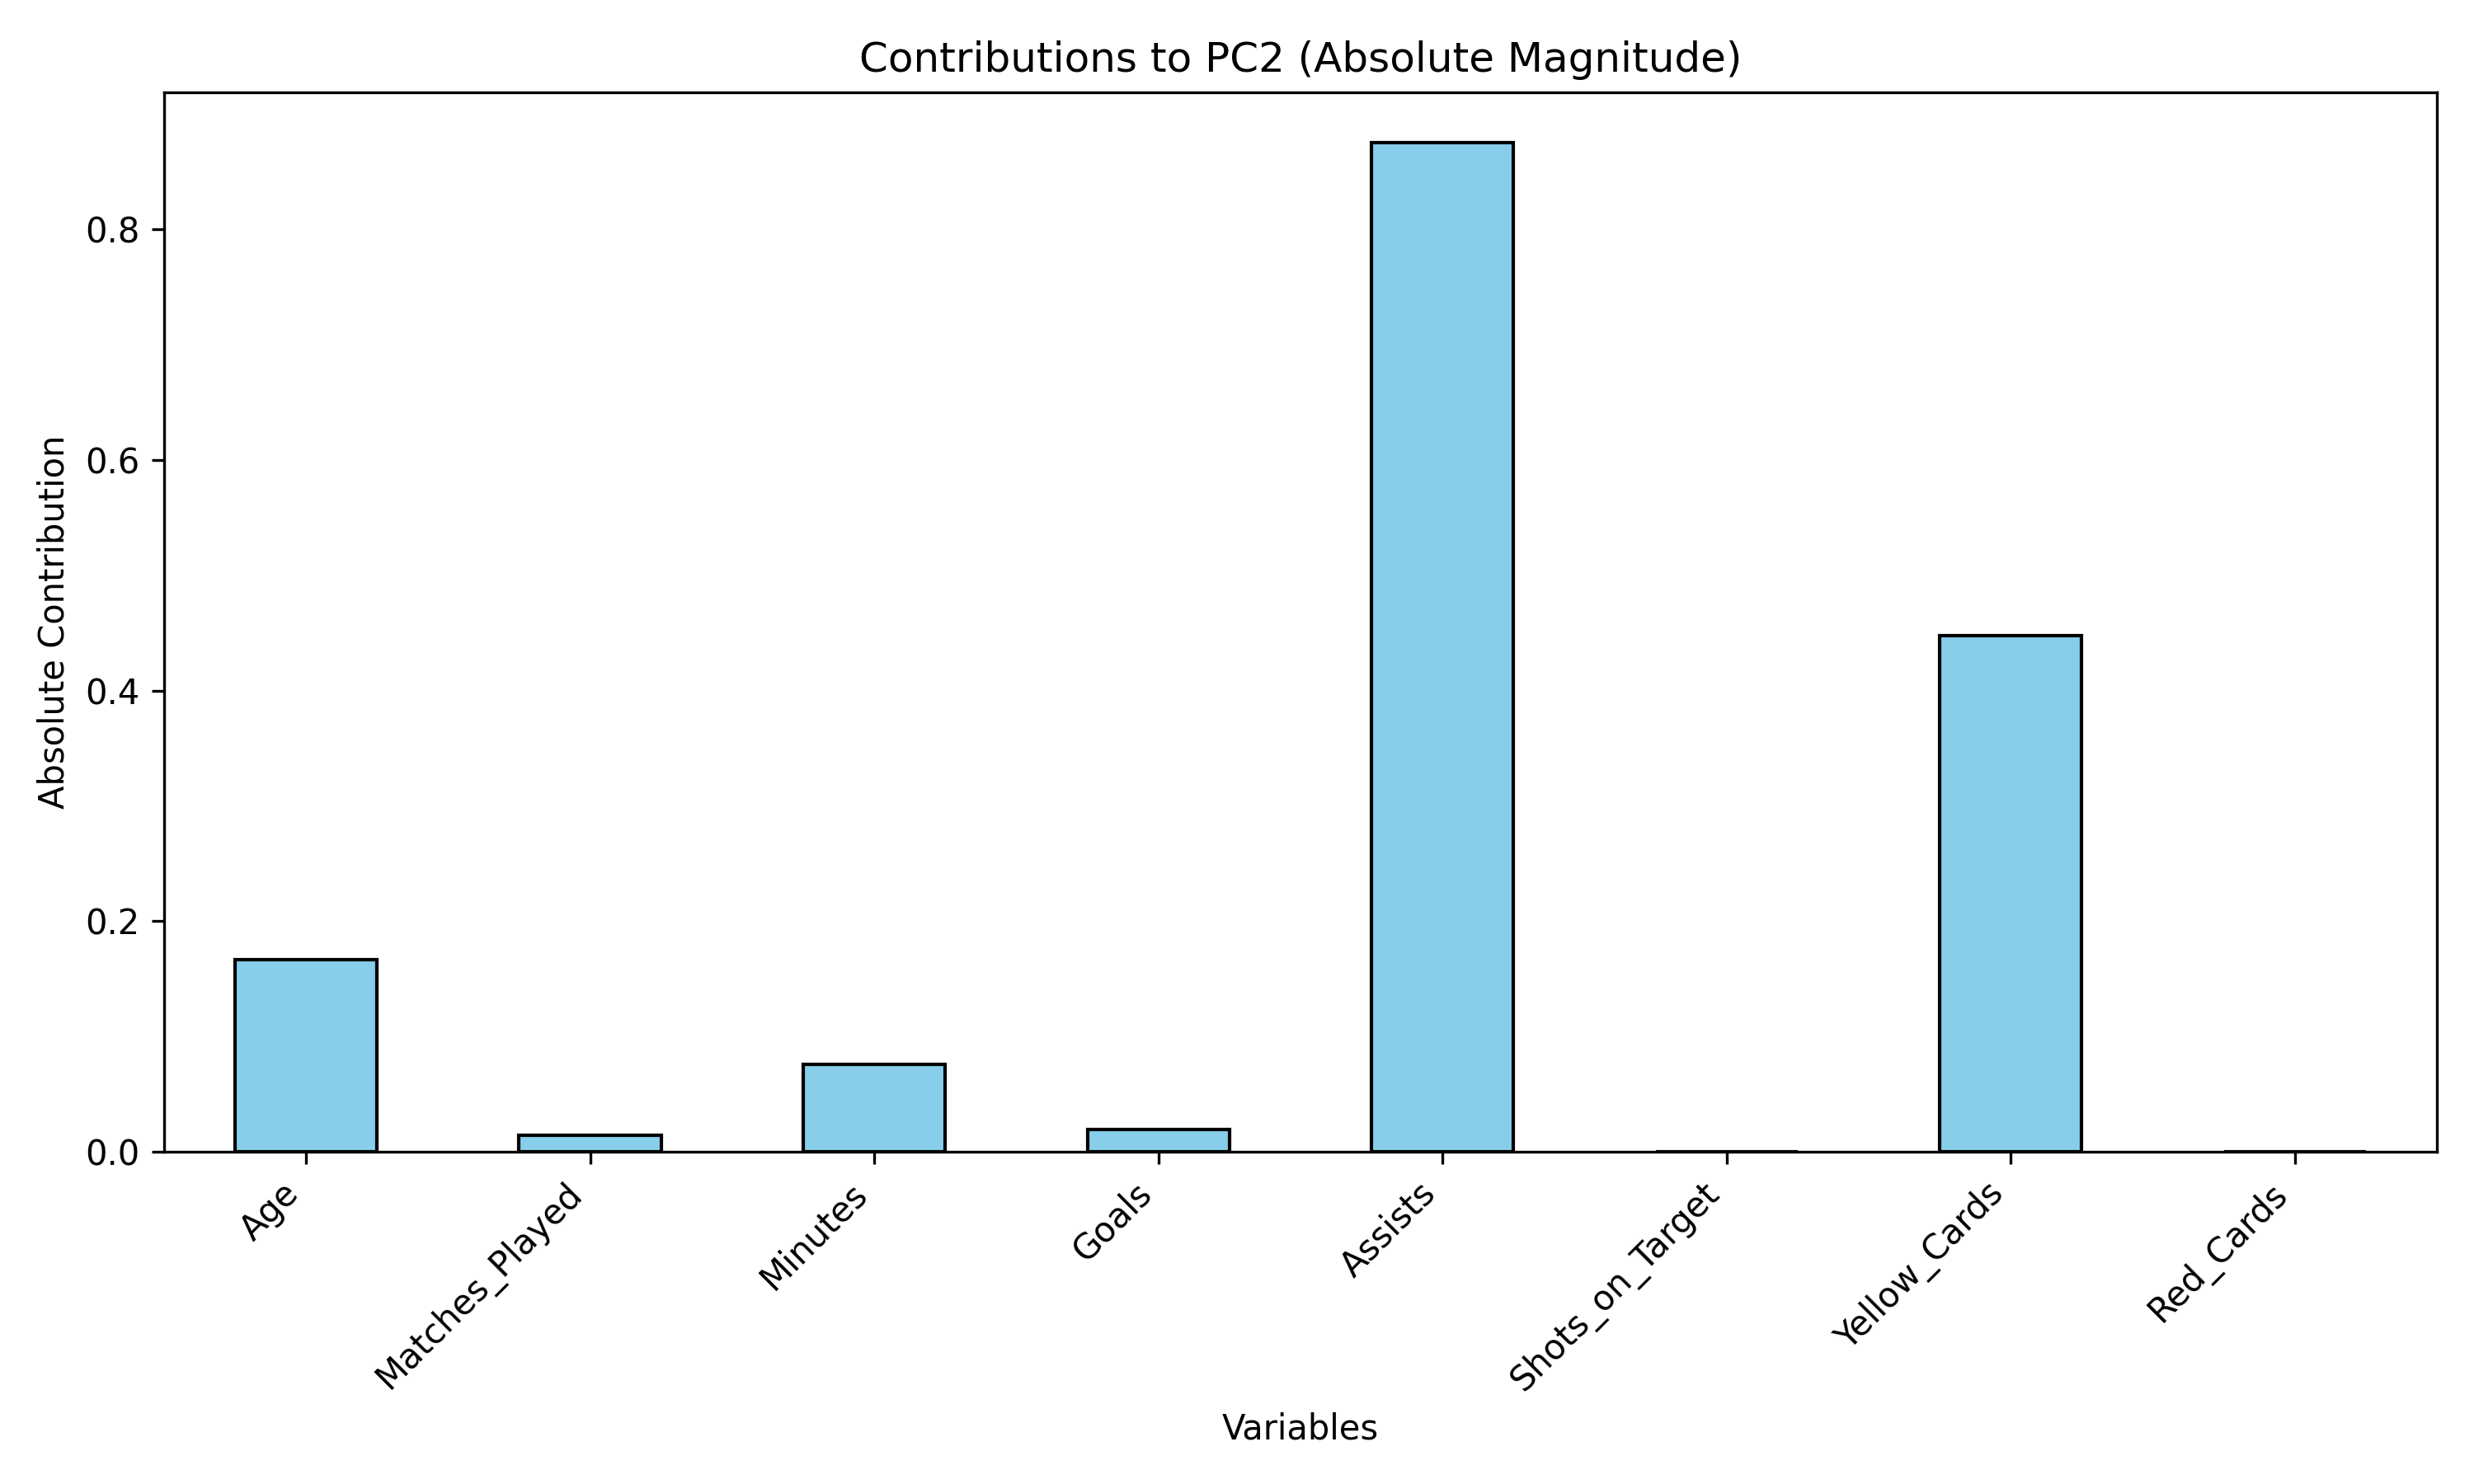
\includegraphics[scale=0.4]{/home/soundskydriver/Documents/topological_data_analysis_mx_league/reports/figures/pca_analysis/contributions_PC2_absolute.png}
				\caption{Contribuciones de las variables al segundo componente principal}
                \label{fig: Figura2}
			\end{figure}
		\end{frame}
        \begin{frame}{Resultados}
			\justifying
            La proyección de los datos en el espacio de las dos primeras componentes principales:
            \begin{figure}[H]
				\centering
				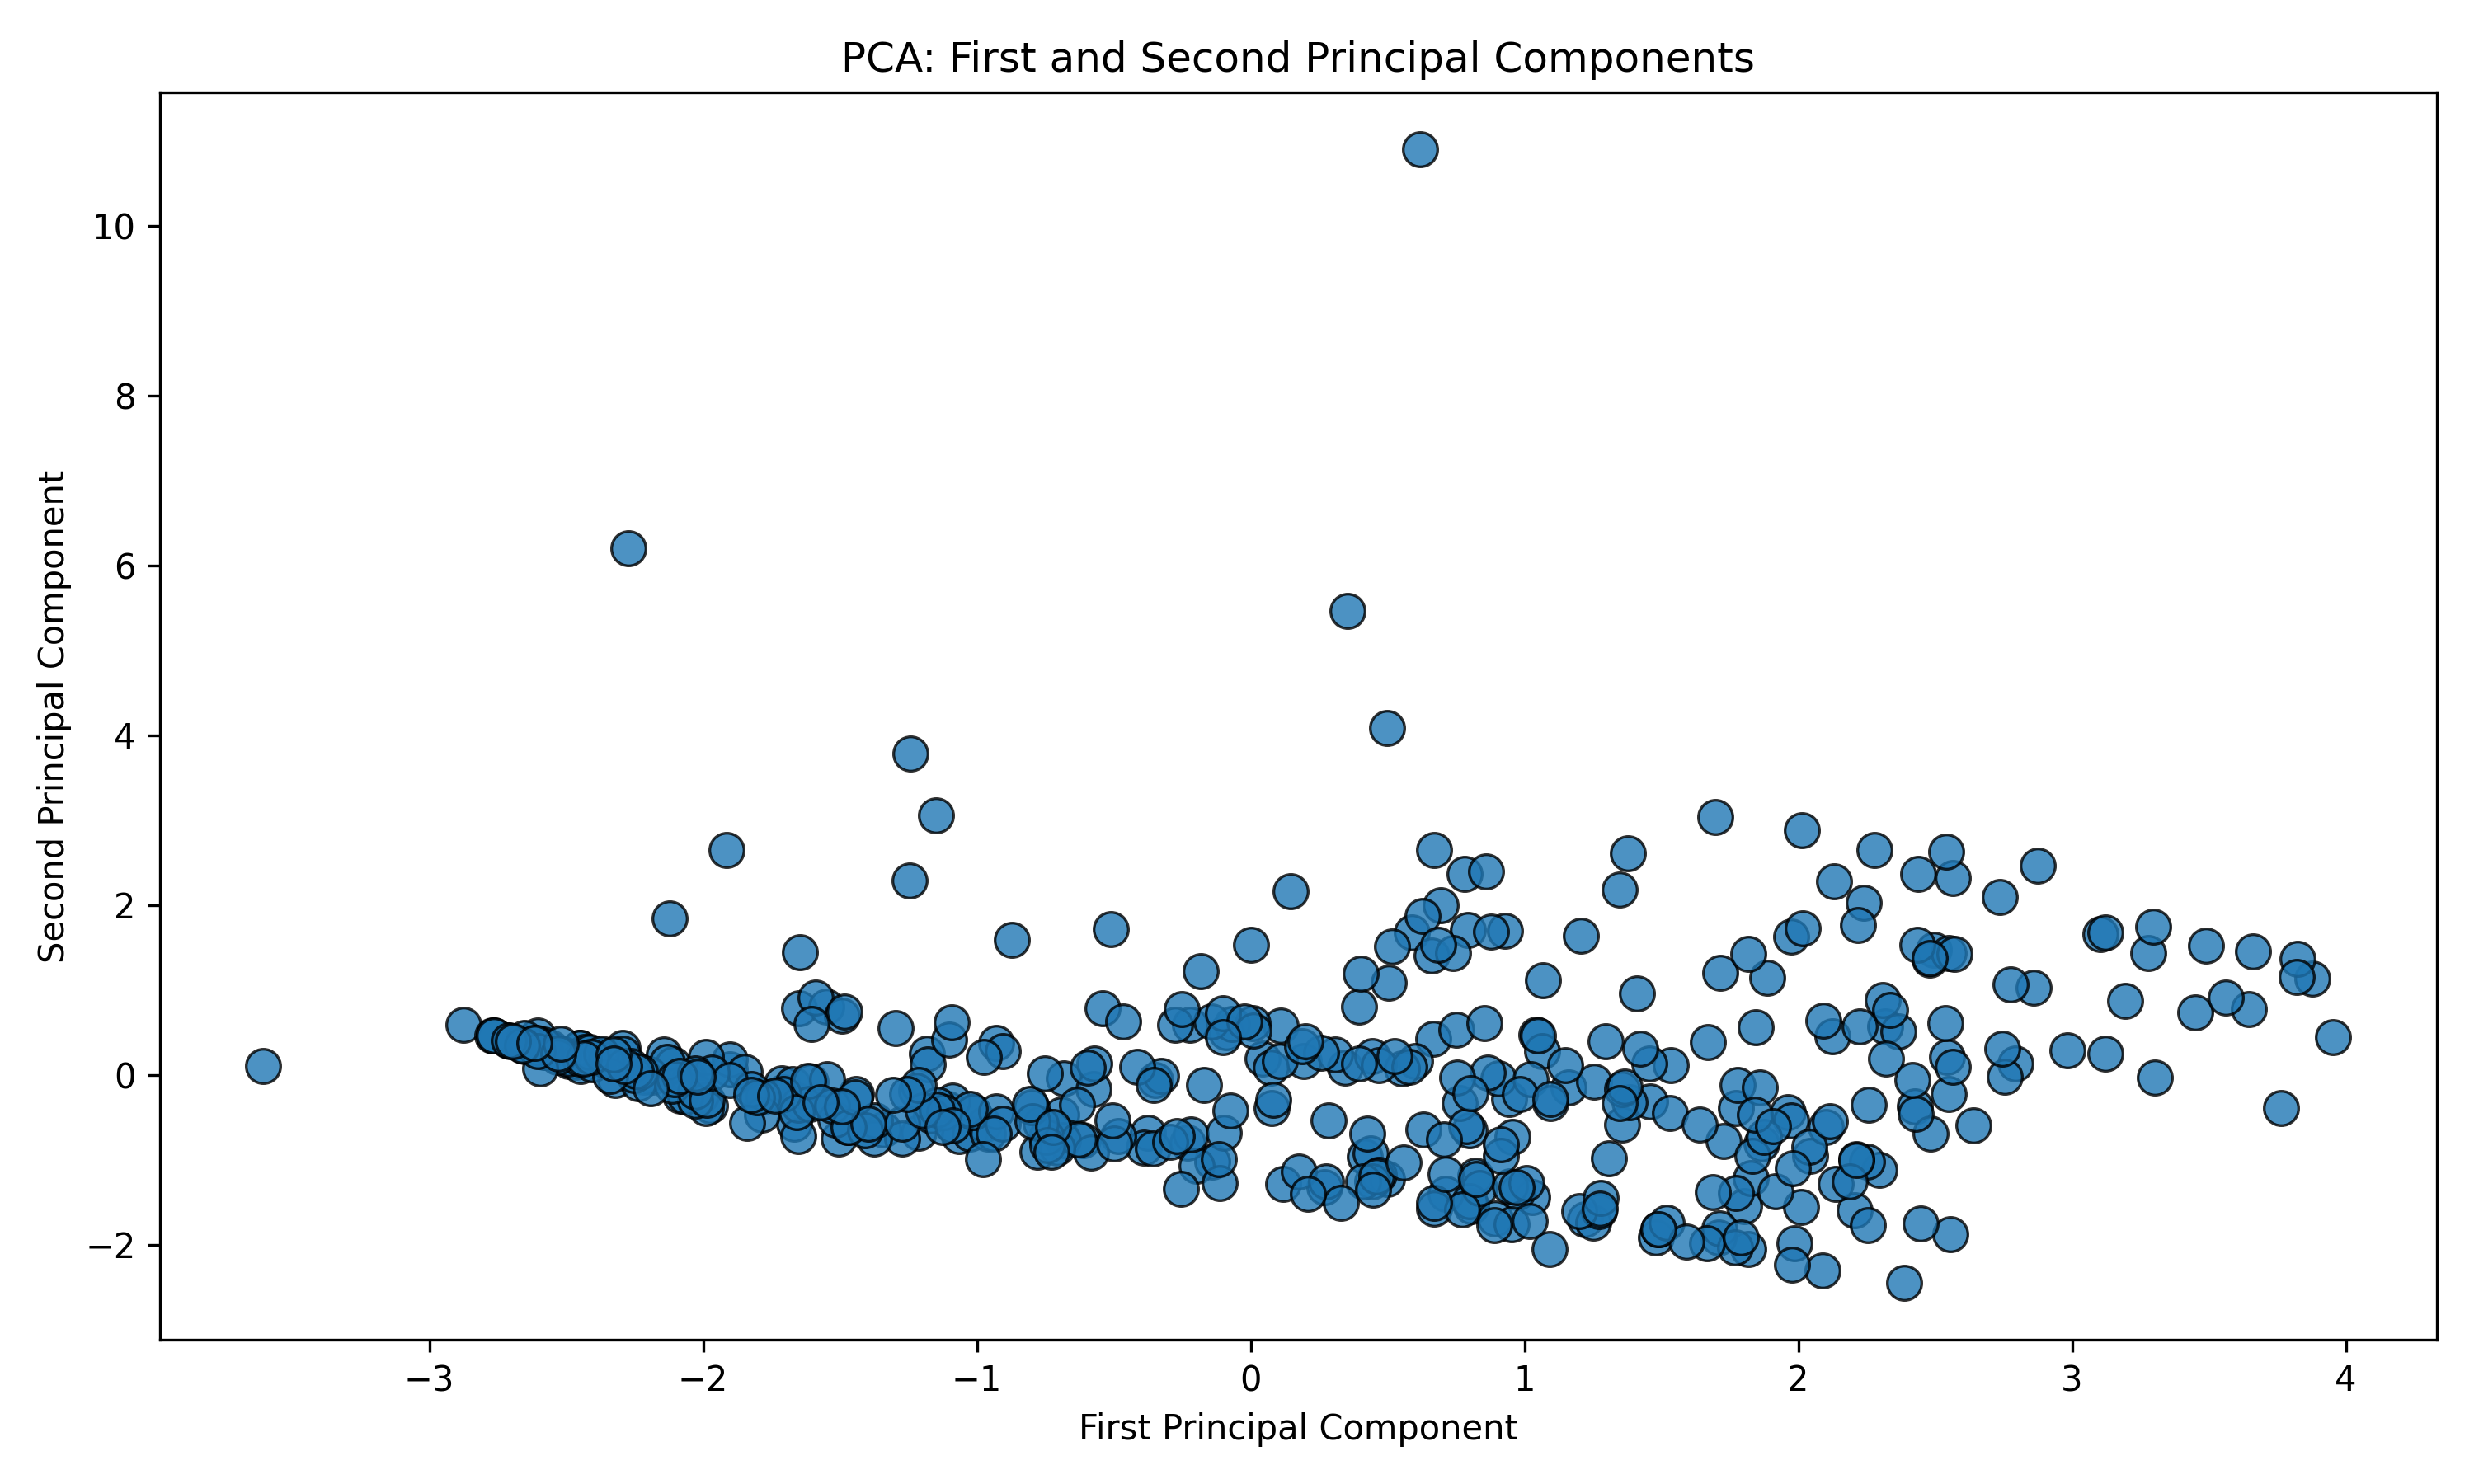
\includegraphics[scale=0.4]{/home/soundskydriver/Documents/topological_data_analysis_mx_league/reports/figures/pca_analysis/pca_projection.png}
				\caption{Contribuciones de las variables al segundo componente principal}
                \label{fig: Figura3}
			\end{figure}
		\end{frame}
        \subsection{Homología Persistente | Barcode Diagram}
        \begin{frame}{Resultados | Homología Persistente}
			\justifying
            La proyección de los datos en el espacio de las dos primeras componentes principales:.
            \begin{figure}[H]
				\centering
				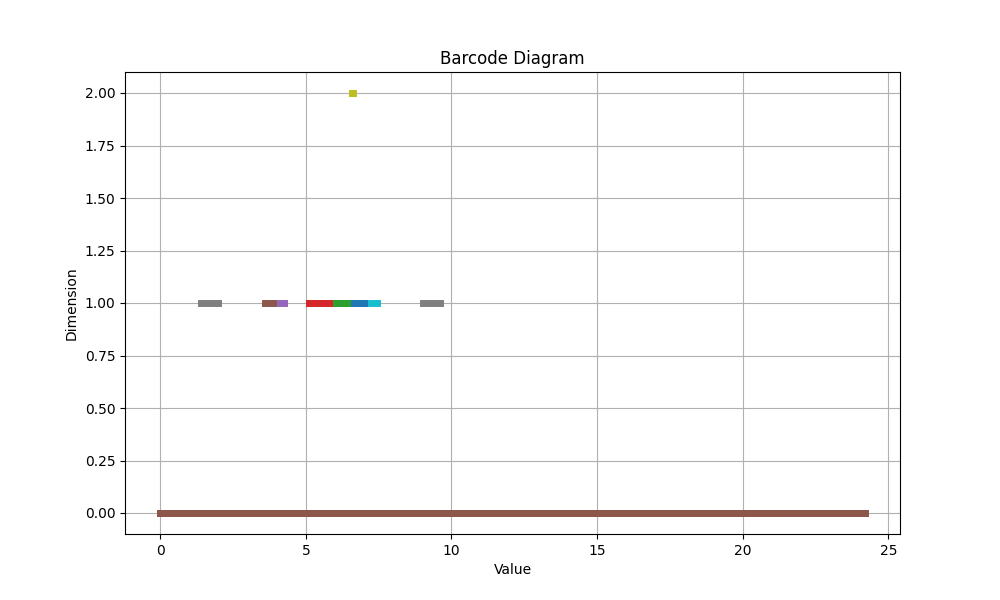
\includegraphics[scale=0.4]{/home/soundskydriver/Documents/topological_data_analysis_mx_league/reports/figures/persistent_homology/barcode_diagram.png}
				\caption{Diagrama de barras de la homología persistente}
                \label{fig: Figura4}
			\end{figure}
        \end{frame}
        \subsection{Homología Persistente | Persistent Diagram}
        \begin{frame}{Resultados | Homología Persistente}
			\justifying
            La proyección de los datos en el espacio de las dos primeras componentes principales:.
            \begin{figure}[H]
				\centering
				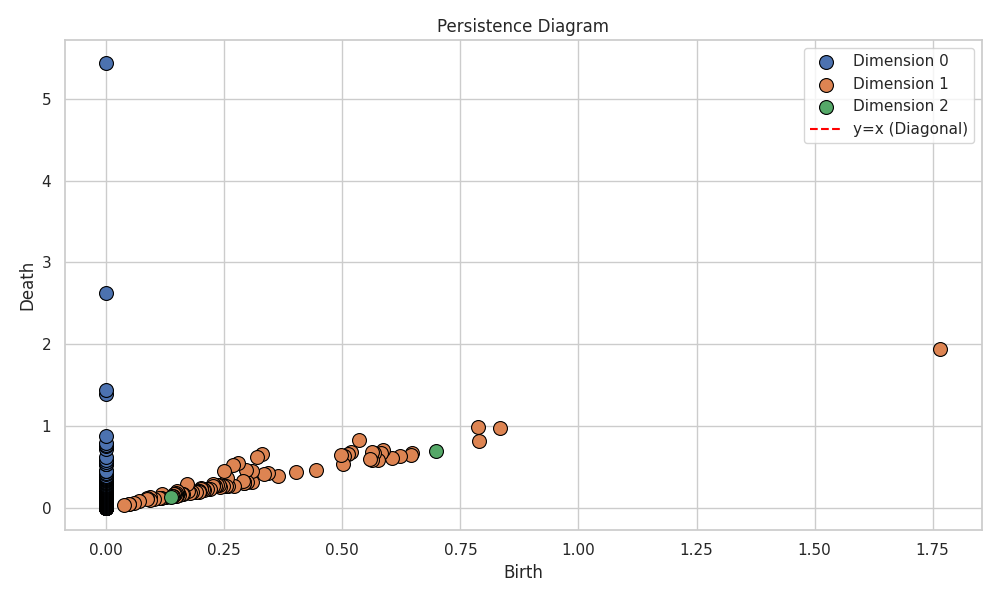
\includegraphics[scale=0.4]{/home/soundskydriver/Documents/topological_data_analysis_mx_league/reports/figures/persistent_homology/persistence_diagram_sns.png}
				\caption{Diagrama persistente de la homología}
                \label{fig: Figura5}
			\end{figure}
        \end{frame}
        \subsection{Algoritmo Mapper | Grafo Topológico}
        \begin{frame}{Resultados | Algoritmo Mapper}
            \justifying
            La proyección de los datos en el espacio de las dos primeras componentes principales:
            \begin{figure}[H]
                \centering
                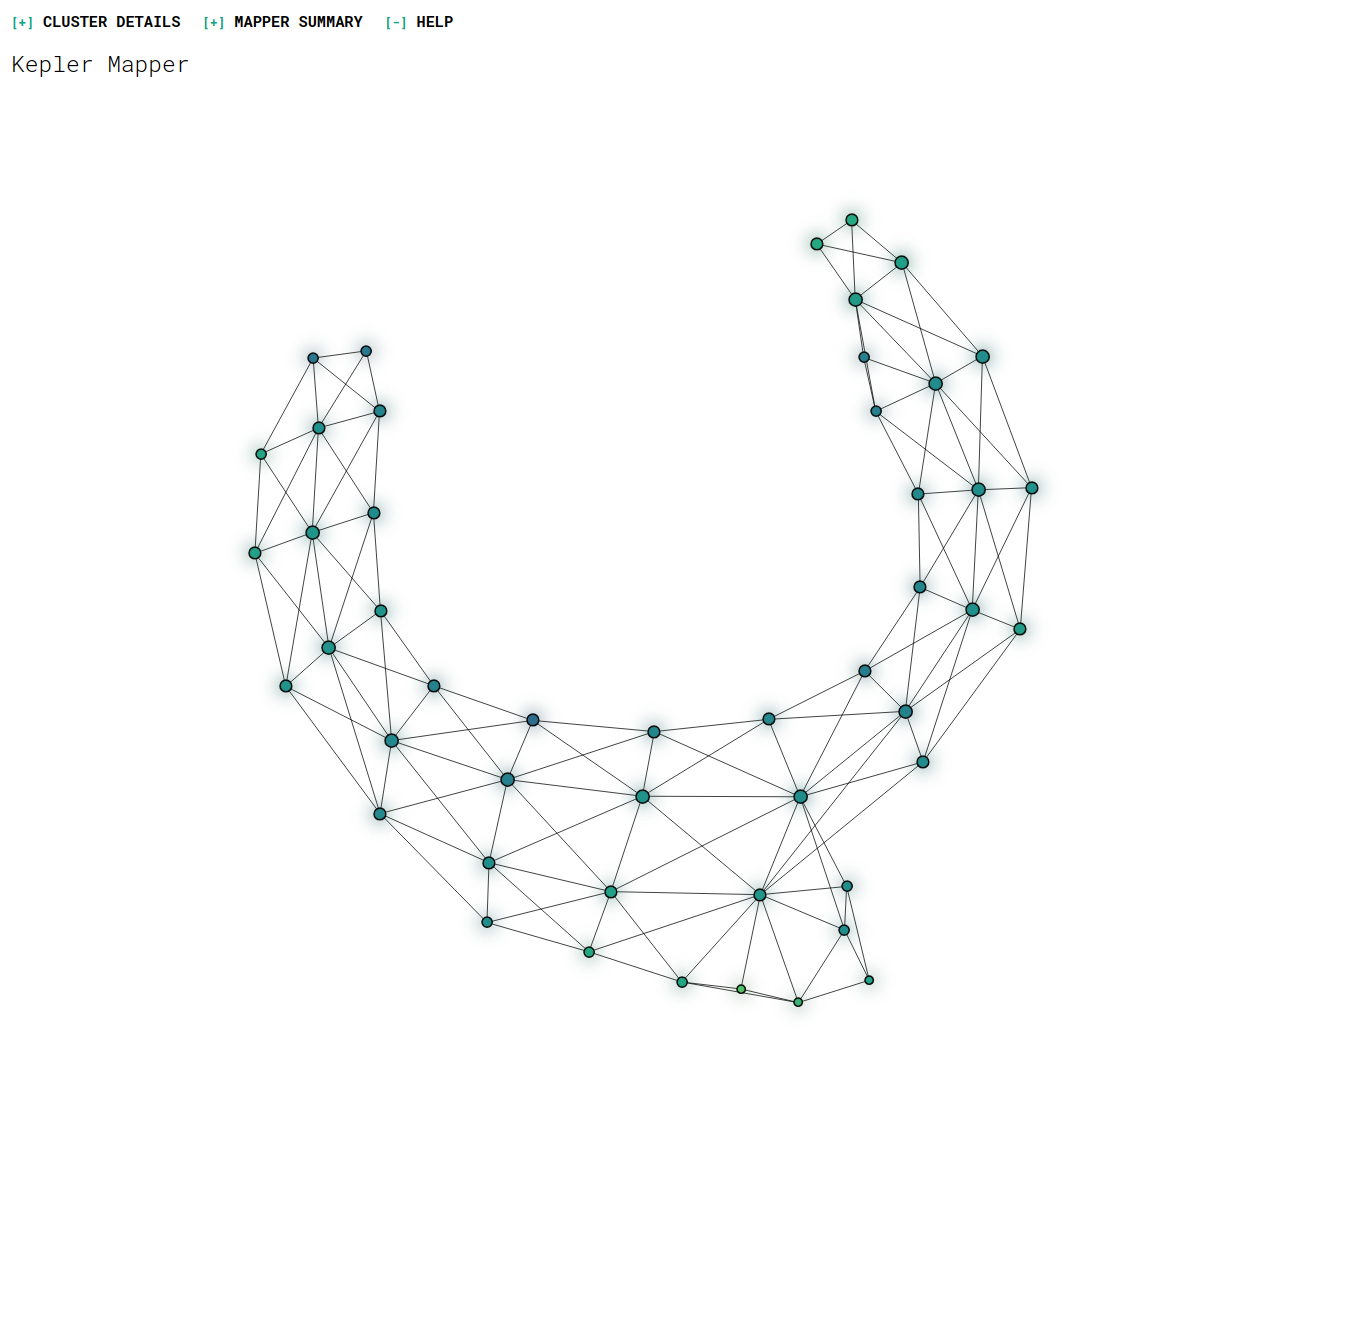
\includegraphics[scale=0.13]{/home/soundskydriver/Documents/topological_data_analysis_mx_league/reports/figures/mapper/Screenshot from 2024-11-28 17-46-00.png}
                \caption{Grafo topológico generado por el algoritmo Mapper}
                \label{fig: Figura6}
            \end{figure}
        \end{frame}

	


\appendix

\begin{frame}{Referencias}
    \begin{itemize}
        \item Lum, P. Y., Singh, G., Lehman, A., Ishkanov, T., Vejdemo-Johansson, M., Alagappan, M., $\cdots$ Carlsson, G. (2013). Extracting insights from the shape of complex data using topology. \textit{Scientific Reports}, 3(1), 1236.
    \end{itemize}
\end{frame}

\end{document}

